\chapter{ResStock Outputs}\label{sec:resstock_outputs}
ResStock produces a range of results around energy, housing characteristics, schedules, emissions, and costs. This section overviews the outputs available in the latest ResStock data release. The data dictionary that summarizes these outputs is available with the \href{https://oedi-data-lake.s3.amazonaws.com/nrel-pds-building-stock/end-use-load-profiles-for-us-building-stock/2025/resstock_amy2018_release_1/data_dictionary.tsv}{data release}.

\section{Building Characteristics}
%Tables - basically our data dictionaries (ideally automated). Data dictionaries are already automated but need heavy QC
The ResStock workflow generates a sample of residential housing units using the conditional distributions and sampling methodology described in Section \ref{sec:sampling_methodology}. Each housing unit sample is specified using a set of characteristics, which include location, housing type, vintage,  heating fuel, building size and geometry, materials, information on the HVAC system, insulation, infiltration, appliances, as well as information on occupant demographics and  behavior. These characteristics are used for the model creation process, but they are also available as metadata associated with the results. The metadata is useful for performing analysis and slicing the data into segments. Some characteristics directly impact the OpenStudio model creation (e.g., wall insulation levels), whereas others are meta-parameters used as tags (e.g., ISO/RTO region) or as characteristics that correlate with other energy-relevant characteristics (e.g., vintage). Each of these characteristics is described in detail in Section \ref{sec:resstock_inputs}, and are summarized in Table \ref{table:hc_output_fields}. In published ResStock datasets, these housing characteristics are the fields that use the ``in'' prefix followed by the housing characteristic name, for example ``in.windows'' for the Windows characteristic. If an upgrade or measure changes a housing characteristic, the post-upgrade characteristic uses the ``upgrade'' prefix, for example ``upgrade.windows.''

Most national ResStock data releases have approximately one sample for every 250 housing units that actually exist in the modeled geography, though this can vary if the sample size is increased or decreased. Taken together, the set of samples describes the housing stock with its intrinsic variety and is used as both an output of ResStock and an input to further steps in the ResStock workflow (see Section \ref{sec:workflow} for more information about the workflow).

Note that ResStock assigns certain characteristics that are not always used. Two examples of this are \textit{cooling setpoint} in housing units with no cooling system, and \textit{clothes washer usage level} in housing units with no clothes washer. This doesn't impact the building energy models, this is merely a mechanism that allows for variability in probability distributions if the schedules are used for an upgrade. These characteristics, however, can lead to confusion because they're preserved in the metadata as being assigned even if they're not modeled. For further discussion see the the BuildStock Batch \href{https://buildstockbatch.readthedocs.io/en/v2023.10.0/project_defn.html#upgrade-scenarios}{Upgrade Scenario} documentation.


\begin{customLongTable}{ |p{6cm}|p{9cm}| }
{ResStock building characteristic output field names and descriptions} {table:hc_output_fields}
{\textbf{Field Name} & \textbf{Field Description}}
        applicability & Whether the upgrade is applicable to this model. Always True for baseline.  \\ \hline
        bldg\_id & The identifier for this model, which can be traced back to the building characteristics input file \\ \hline
        completed\_status & Whether the simulation for this model was successful or not \\ \hline
        in.ahs\_region & American Housing Survey region \\ \hline
        in.aiannh\_area & The sample is or is not located in census-designated American Indian/Alaska Native/Native Hawaiian Area \\ \hline
        in.air\_leakage\_to\_outside\_ach50 & Nominal air infiltration rate \\ \hline
        in.applicable & Whether the upgrade is applicable to this model. Always True for baseline.  \\ \hline
        in.area\_median\_income & Area median income of the household occupying the housing unit \\ \hline
        in.ashrae\_iecc\_climate\_zone\_2004 & IECC climate zone according to ASHRAE 169 in 2004 and IECC in 2012 \\ \hline
        in.ashrae\_iecc\_climate\_zone\_2004\_sub\_cz\_split & Climate zone according to ASHRAE 169 in 2004 and IECC in 2012, where climate zone 2A is split between counties in TX, LA versus FL, GA, AL, and MS and climate zone 1A is split between FL and HI\\ \hline
        in.bathroom\_spot\_vent\_hour & Bathroom spot ventilation daily start hour \\ \hline
        in.battery & The presence, size, location, and efficiency of an on-site battery (not modeled in 2024.2 dataset) \\ \hline
        in.bedrooms & Number of bedrooms \\ \hline
        in.building\_america\_climate\_zone & Building America climate zone \\ \hline
        in.buildstock\_csv\_path & Where the building characteristics file is located \\ \hline
        in.cec\_climate\_zone & California Energy Code climate zone \\ \hline
        in.ceiling\_fan & Presence and energy usage of ceiling fans at medium speed \\ \hline
        in.census\_division & 2010 U.S. Census Division \\ \hline
        in.census\_division\_recs & Census Division as used in RECS 2015 \\ \hline
        in.census\_region & 2010 U.S. Census Region \\ \hline
        in.city & The census-designated city where the sample is located \\ \hline
        in.clothes\_dryer & The presence, rated efficiency, and fuel type of the clothes dryer in the housing unit \\ \hline
        in.clothes\_dryer\_usage\_level & Clothes dryer energy usage level multiplier \\ \hline
        in.clothes\_washer & Presence and rated efficiency of the clothes washer \\ \hline
        in.clothes\_washer\_presence & Presence of clothes washer \\ \hline
        in.clothes\_washer\_usage\_level & Clothes washer energy usage level multiplier \\ \hline
        in.cooking\_range & Presence and fuel type of the cooking range \\ \hline
        in.cooking\_range\_usage\_level & Cooking range energy usage level multiplier \\ \hline
        in.cooling\_setpoint & Base cooling setpoint with no offset applied \\ \hline
        in.cooling\_setpoint\_has\_offset & Presence of cooling setpoint offset \\ \hline
        in.cooling\_setpoint\_offset\_magnitude & The magnitude of cooling setpoint offset \\ \hline
        in.cooling\_setpoint\_offset\_period & The period during which the cooling setpoint offset is applied \\ \hline
        in.cooling\_unavailable\_days & The number of days in a year the cooling system is unavailable. \\ \hline
        in.cooling\_unavailable\_period & The time during the year when the cooling system is unavailable. \\ \hline
        in.corridor & Type of corridor \\ \hline
        in.county & County GISJOIN identifier \\ \hline
        in.county\_and\_puma & The GISJOIN identifier for the County and the PUMA that the sample is located \\ \hline
        in.county\_metro\_status & Whether the county is part of a census-defined metro area \\ \hline
        in.county\_name & The name of the county the building is located in \\ \hline
        in.dehumidifier & Presence, water removal rate, and humidity setpoint of dehumidifier (not modeled in 2024.2 dataset) \\ \hline
        in.dishwasher & Presence and rated efficiency of dishwasher \\ \hline
        in.dishwasher\_usage\_level & Dishwasher energy usage level multiplier \\ \hline
        in.door\_area & Area of exterior doors \\ \hline
        in.doors & Exterior door material and properties \\ \hline
        in.duct\_leakage\_and\_insulation & Duct insulation and leakage to outside from the portion of ducts in unconditioned spaces \\ \hline
        in.duct\_location & Location of duct system \\ \hline
        in.eaves & Depth of roof eaves \\ \hline
        in.electric\_panel\_breaker\_space\_total\_count & Total breaker spaces on electric panel \\ \hline
        in.electric\_panel\_service\_rating..a & Electrical panel service or max current rating (A) \\ \hline
        in.electric\_panel\_service\_rating\_bin..a & Electrical panel service or max current rating in bins (A) \\ \hline
        in.electric\_vehicle\_battery & The type of battery used by EV \\ \hline
        in.electric\_vehicle\_charge\_at\_home & Percentage of EV charging that occurs at home \\ \hline
        in.electric\_vehicle\_charger & The type of charger used by EV \\ \hline
        in.electric\_vehicle\_miles\_traveled & Annual miles traveled by EV \\ \hline
        in.electric\_vehicle\_outlet\_access & The type of outlet access available for EV \\ \hline
        in.electric\_vehicle\_ownership & Whether the EV is present or not \\ \hline
        in.energystar\_climate\_zone\_2023 & Climate zones for windows, doors, and skylights per ENERGY STAR guidelines as of 2023 \\ \hline
        in.federal\_poverty\_level & Federal poverty level of the household occupying the housing unit \\ \hline
        in.generation\_and\_emissions\_assessment\_region & Generation and carbon emissions assessment (GEA) region from Cambium 2023 \\ \hline
        in.geometry\_attic\_type & Type of attic \\ \hline
        in.geometry\_building\_horizontal\_location\_mf & Location of the multifamily unit horizontally within the building (left, middle, right) \\ \hline
        in.geometry\_building\_horizontal\_location\_sfa & Location of the single-family attached unit horizontally within the building (left, middle, right) \\ \hline
        in.geometry\_building\_level\_mf & Location of the multifamily unit vertically within the building (bottom, middle, top) \\ \hline
        in.geometry\_building\_number\_units\_mf & Number of units in the multifamily building in which the housing unit is located \\ \hline
        in.geometry\_building\_number\_units\_sfa & Number of units in the single-family attached building in which housing unit is located \\ \hline
        in.geometry\_building\_type\_acs & American Community Survey building type \\ \hline
        in.geometry\_building\_type\_height & RECS 2009 building type with multifamily buildings split out by low-rise, mid-rise, and high-rise \\ \hline
        in.geometry\_building\_type\_recs & PUMS 2019 building type \\ \hline
        in.geometry\_floor\_area & Finished floor area bin (American Housing Survey) \\ \hline
        in.geometry\_floor\_area\_bin & Finished floor area bin \\ \hline
        in.geometry\_foundation\_type & Type of building foundation \\ \hline
        in.geometry\_garage & Presence and size of an attached garage \\ \hline
        in.geometry\_space\_combination & Valid combinations of building type, building level MF, attic, foundation, and garage \\ \hline
        in.geometry\_stories & Number of building stories in which housing unit is located \\ \hline
        in.geometry\_stories\_low\_rise & Number of building stories for low rise building in which housing unit is located \\ \hline
        in.geometry\_story\_bin & The building in which housing unit is located has 8 or more versus fewer than 8 stories \\ \hline
        in.geometry\_wall\_exterior\_finish & Exterior wall finish material and color \\ \hline
        in.geometry\_wall\_type & Exterior wall material \\ \hline
        in.ground\_thermal\_conductivity & The thermal conductivity of the ground using in foundation and geothermal heat pump heat transfer calculations \\ \hline
        in.has\_pv & Presence of rooftop PV \\ \hline
        in.heating\_fuel & Fuel used for primary heating \\ \hline
        in.heating\_setpoint & Baseline heating setpoint with no offset applied \\ \hline
        in.heating\_setpoint\_has\_offset & Presence of heating setpoint offset \\ \hline
        in.heating\_setpoint\_offset\_magnitude & The magnitude of heating setpoint offset \\ \hline
        in.heating\_setpoint\_offset\_period & The period during which the heating setpoint offset is applied \\ \hline
        in.heating\_unavailable\_days & The number of days in a year the heating system is unavailable. \\ \hline
        in.heating\_unavailable\_period & The time during the year when the heating system is unavailable. \\ \hline
        in.holiday\_lighting & Presence, energy usage, and schedule of holiday lighting \\ \hline
        in.hot\_water\_distribution & Hot water piping material and insulation level \\ \hline
        in.hot\_water\_fixtures & Hot water fixture usage and flow levels \\ \hline
        in.household\_has\_tribal\_persons & The housing unit houses at least one Tribal person \\ \hline
        in.hvac\_cooling\_autosizing\_factor & The additional safety factor applied to the HVAC system cooling capacity \\ \hline
        in.hvac\_cooling\_efficiency & Presence and efficiency of cooling system \\ \hline
        in.hvac\_cooling\_partial\_space\_conditioning & The fraction of the finished floor area that is cooled by the cooling system \\ \hline
        in.hvac\_cooling\_type & Presence and type of cooling system \\ \hline
        in.hvac\_has\_ducts & Presence of ducts \\ \hline
        in.hvac\_has\_shared\_system & Presence of shared HVAC system \\ \hline
        in.hvac\_has\_zonal\_electric\_heating & Presence of electric baseboard heating \\ \hline
        in.hvac\_heating\_autosizing\_factor & The additional safety factor applied to the HVAC system heating capacity \\ \hline
        in.hvac\_heating\_efficiency & Presence and efficiency of primary heating system \\ \hline
        in.hvac\_heating\_type & Presence and type of primary heating system \\ \hline
        in.hvac\_heating\_type\_and\_fuel & Presence, type, and fuel of primary heating system \\ \hline
        in.hvac\_secondary\_heating\_efficiency & Presence and efficiency of secondary heating system \\ \hline
        in.hvac\_secondary\_heating\_fuel & Secondary HVAC system heating type and fuel \\ \hline
        in.hvac\_secondary\_heating\_heating\_type & The type of the secondary heating system \\ \hline
        in.hvac\_secondary\_heating\_partial\_space\_conditioning & Fraction of heat load served by secondary heating system \\ \hline
        in.hvac\_secondary\_heating\_type & Secondary HVAC system heating type \\ \hline
        in.hvac\_shared\_efficiencies & Presence and efficiency of shared HVAC system \\ \hline
        in.hvac\_system\_is\_faulted & Not used \\ \hline
        in.hvac\_system\_is\_scaled & Not used \\ \hline
        in.hvac\_system\_single\_speed\_ac\_airflow & Not used \\ \hline
        in.hvac\_system\_single\_speed\_ac\_charge & Not used \\ \hline
        in.hvac\_system\_single\_speed\_ashp\_airflow & Not used \\ \hline
        in.hvac\_system\_single\_speed\_ashp\_charge & Not used \\ \hline
        in.income & Income bin of the household occupying the housing unit \\ \hline
        in.income\_recs\_2015 & Income bin of the household occupying the housing unit aligned with the 2015 U.S. EIA RECS \\ \hline
        in.income\_recs\_2020 & Income bin of the household occupying the housing unit aligned with the 2020 U.S. EIA RECS \\ \hline
        in.infiltration & Air leakage rates for the living and garage spaces \\ \hline
        in.insulation\_ceiling & Ceiling insulation level (between the living space and unconditioned attic) \\ \hline
        in.insulation\_floor & Floor insulation level \\ \hline
        in.insulation\_foundation\_wall & Foundation walls insulation level \\ \hline
        in.insulation\_rim\_joist & Insulation level for rim joists \\ \hline
        in.insulation\_roof & Finished roof insulation level between roof and conditioned space \\ \hline
        in.insulation\_slab & Slab insulation level \\ \hline
        in.insulation\_wall & Wall construction type and insulation level \\ \hline
        in.interior\_shading & Fraction of the window area shaded from the interior in the summer and winter \\ \hline
        in.iso\_rto\_region & ISO or RTO region \\ \hline
        in.lighting & Fraction of lighting types \\ \hline
        in.lighting\_interior\_use & Interior lighting usage relative to the national average \\ \hline
        in.lighting\_other\_use & Exterior and garage lighting usage relative to the national average \\ \hline
        in.location\_region & Custom ResStock region \\ \hline
        in.mechanical\_ventilation & Mechanical ventilation type and efficiency \\ \hline
        in.metropolitan\_and\_micropolitan\_statistical\_area & The census metropolitan or micropolitan statistical area where this model is located \\ \hline
        in.misc\_extra\_refrigerator & Presence and rated efficiency of extra refrigerator \\ \hline
        in.misc\_freezer & Presence and rated efficiency of standalone freezer \\ \hline
        in.misc\_gas\_fireplace & Presence of gas fireplace \\ \hline
        in.misc\_gas\_grill & Presence of gas grill \\ \hline
        in.misc\_gas\_lighting & Presence of exterior gas lighting \\ \hline
        in.misc\_hot\_tub\_spa & Presence and fuel type of hot tub \\ \hline
        in.misc\_pool & Presence of pool \\ \hline
        in.misc\_pool\_heater & Presence and fuel type of pool heater \\ \hline
        in.misc\_pool\_pump & Presence and size of pool pump \\ \hline
        in.misc\_well\_pump & Presence and efficiency of well pump \\ \hline
        in.natural\_ventilation & Schedule of natural ventilation from windows \\ \hline
        in.neighbors & Presence and distance between the housing unit and the nearest neighbors to the left and right. \\ \hline
        in.occupants & The number of occupants living in the housing unit \\ \hline
        in.orientation & Orientation of the building \\ \hline
        in.overhangs & Presence, depth, and location of window overhangs \\ \hline
        in.plug\_load\_diversity & Plug load diversity multiplier relative to the national average \\ \hline
        in.plug\_loads & Plug load usage level relative to the national average \\ \hline
        in.puma & The  2010 U.S. Census PUMA where the sample is located \\ \hline
        in.puma\_metro\_status & The PUMA metropolitan status \\ \hline
        in.pv\_orientation & Presence and orientation of rooftop PV system \\ \hline
        in.pv\_system\_size & Presence and size of rooftop PV system \\ \hline
        in.radiant\_barrier & Presence of radiant barrier in attic \\ \hline
        in.range\_spot\_vent\_hour & Range spot ventilation daily start hour \\ \hline
        in.reeds\_balancing\_area & Regional Energy Deployment System Model balancing area \\ \hline
        in.refrigerator & The presence and rated efficiency of the primary refrigerator \\ \hline
        in.refrigerator\_usage\_level & Refrigerator energy usage level multiplier \\ \hline
        in.representative\_income & The income assumed for the household in this unit for energy burden calculation \\ \hline
        in.roof\_material & Roof material type \\ \hline
        in.solar\_hot\_water & Presence, size, and location of solar hot water system \\ \hline
        in.sqft..ft2 & Finished floor area of the representative housing unit \\ \hline
        in.state & State \\ \hline
        in.state\_metro\_median\_income & The census-supplied median income for households in the metro area where this unit is located. \\ \hline
        in.tenure & The tenancy (owner or renter) of the household occupying the housing unit \\ \hline
        in.units\_represented & Number of housing units the building model represents (this field is no longer used) \\ \hline
        in.usage\_level & Usage of major appliances relative to the national average \\ \hline
        in.upgrade\_name & Name of the upgrade applied, or Baseline when no upgrade is applied \\ \hline

        in.vacancy\_status & Presence of occupants \\ \hline
        in.vintage & Range in which the building was constructed \\ \hline
        in.vintage\_acs & Range in which the building was constructed using ACS bins \\ \hline
        in.water\_heater\_efficiency & Efficiency, type, and heating fuel of water heater \\ \hline
        in.water\_heater\_fuel & Water heater fuel \\ \hline
        in.water\_heater\_in\_unit & Individual water heater present or not present in the housing unit that solely serves the specific housing unit \\ \hline
        in.water\_heater\_location & Water heater location for the housing unit if applicable \\ \hline
        in.weather\_file\_city & City of weather file \\ \hline

        in.window\_areas & Window to wall ratios of the front, back, left, and right walls  \\ \hline
        in.windows & Construction type and efficiency levels of windows \\
\end{customLongTable}

In addition to the housing characteristics themselves, several other ResStock outputs receive the ``in.'' prefix. These are inputs that are not provided as housing characteristics, but that are necessary inputs to the model. Most of these values are specified in the \href{https://github.com/NREL/resstock/blob/v3.2.0-2024.2/project_national/EUSSRR2_project_500k_AMY2018.yml}{project configuration file}.

\begin{customLongTable}{ |p{6cm}|p{9cm}| }
{ResStock building characteristic output field names and descriptions} {table:supplmentary_input_fields}
{\textbf{Field Name} & \textbf{Field Description}}

        in.emissions\_electricity\_folders & Relative paths of electricity emissions factor schedule files with hourly values. Paths are relative to the resources folder. If multiple scenarios, use a comma-separated list. File names must contain GEA region names. \\ \hline
        in.emissions\_electricity\_units & Electricity emissions factors units. If multiple scenarios, use a comma-separated list. Only lb/MWh and kg/MWh are allowed. \\ \hline
        in.emissions\_electricity\_values\_or\_filepaths & Electricity emissions factors values, specified as either an annual factor or an absolute/relative path to a file with hourly factors. If multiple scenarios, use a comma-separated list. \\ \hline
        in.emissions\_fossil\_fuel\_units & Fossil fuel emissions factors units. If multiple scenarios, use a comma-separated list. Only lb/MBtu and kg/MBtu are allowed. \\ \hline
        in.emissions\_fuel\_oil\_values & Fuel oil emissions factors values, specified as an annual factor. If multiple scenarios, use a comma-separated list. \\ \hline
        in.emissions\_natural\_gas\_values & Natural gas emissions factors values, specified as an annual factor. If multiple scenarios, use a comma-separated list. \\ \hline
        in.emissions\_propane\_values & Propane emissions factors values, specified as an annual factor. If multiple scenarios, use a comma-separated list. \\ \hline
        in.emissions\_scenario\_names & Names of emissions scenarios. If multiple scenarios, use a comma-separated list. \\ \hline
        %in.emissions\_types & Types of emissions (e.g., CO2e, NOx, etc.). If multiple scenarios, use a comma-separated list \\ \hline
        in.simulation\_control\_run\_period\_begin\_day\_of\_month & The starting day of the starting month for the annual run period. \\ \hline
        in.simulation\_control\_run\_period\_begin\_month & The starting month number (1 = January, 2 = February, etc.) for the annual run period. \\ \hline
        in.simulation\_control\_run\_period\_calendar\_year & The calendar year that determines the start day of week. \\ \hline
        in.simulation\_control\_run\_period\_end\_day\_of\_month & The ending day of the ending month for the annual run period. \\ \hline
        in.simulation\_control\_run\_period\_end\_month & The end month number (1 = January, 2 = February, etc.) for the annual run period. \\ \hline
        in.simulation\_control\_timestep & Value must be a divisor of 60. \\ \hline

        in.utility\_bill\_detailed\_filepaths & n/a \\ \hline
        in.utility\_bill\_electricity\_filepaths & n/a \\ \hline
        in.utility\_bill\_electricity\_fixed\_charges & Electricity utility bill monthly fixed charges. If multiple scenarios, use a comma-separated list. \\ \hline
        in.utility\_bill\_electricity\_marginal\_rates & Electricity utility bill marginal rates. If multiple scenarios, use a comma-separated list. \\ \hline
        in.utility\_bill\_fuel\_oil\_fixed\_charges & Fuel oil utility bill monthly fixed charges. If multiple scenarios, use a comma-separated list. \\ \hline
        in.utility\_bill\_fuel\_oil\_marginal\_rates & Fuel oil utility bill marginal rates. If multiple scenarios, use a comma-separated list. \\ \hline
        in.utility\_bill\_natural\_gas\_fixed\_charges & Natural gas utility bill monthly fixed charges. If multiple scenarios, use a comma-separated list. \\ \hline
        in.utility\_bill\_natural\_gas\_marginal\_rates & Natural gas utility bill marginal rates. If multiple scenarios, use a comma-separated list. \\ \hline
        in.utility\_bill\_propane\_fixed\_charges & Propane utility bill monthly fixed charges. If multiple scenarios, use a comma-separated list. \\ \hline
        in.utility\_bill\_propane\_marginal\_rates & Propane utility bill marginal rates. If multiple scenarios, use a comma-separated list. \\ \hline
        in.utility\_bill\_scenario\_names & Names of utility bill scenarios. If multiple scenarios, use a comma-separated list. If multiple scenarios, use a comma-separated list. \\ \hline
        in.utility\_bill\_simple\_filepaths & Relative paths of simple utility rates. Paths are relative to the resources folder. If multiple scenarios, use a comma-separated list. \\ \hline

        in.weather\_file\_latitude & Latitude of location of weather file. \\ \hline
        in.weather\_file\_longitude & Longitude of location of weather file. \\ \hline
    \end{customLongTable}

\section{Energy Consumption by Fuel and End Use}
The ResStock workflow models each housing unit sample in OpenStudio and EnergyPlus to produce energy consumption of each model at subhourly time steps and then processes the results into ResStock outputs. These outputs are produced by fuel type (e.g., electricity, natural gas) and end use (e.g., lighting, heating). Totals are calculated for each fuel and for all fuels combined. For electricity and all fuels combined, net totals are also calculated, which incorporate the impacts of on-site photovoltaics. The full list of energy consumption outputs from the ResStock workflow is available in Table \ref{table:results_output_fields}. Note that to date, ResStock has included only consumption of electricity, natural gas, propane, and fuel oil---excluding on-site consumption, wood, coal, or other fuels in its modeling, although the workflow is set up to include these additional fuels. Future releases will likely include wood.

As an output, the energy consumption results are all preceded with an ``out.'' prefix, followed by either the fuel type (e.g., ``out.electricity.'') or ``total.'' if it is an aggregate of all fuel types, and then the end use, ``net.''  or ``total.'' if it is an aggregate of all end uses in that fuel type.
%%%% Bill calculations are really confusing and need to be better covered either here or OS-HPXML (or both). OS-HPXML documentation is lacking

\begin{customLongTable}{ |p{6cm}|p{1.5cm}|p{7cm}| }
{ResStock energy output field names, units, and descriptions} {table:results_output_fields}
{\textbf{Field Name} & \textbf{Units} & \textbf{Field Description}}
        out.electricity.ceiling\_fan.energy\_consumption..kwh & kWh & Electricity consumed by ceiling fans \\ \hline
        out.electricity.clothes\_dryer.energy\_consumption..kwh & kWh & Electricity consumed by clothes dryers \\ \hline
        out.electricity.clothes\_washer.energy\_consumption..kwh & kWh & Electricity consumed by clothes washers \\ \hline
        out.electricity.cooling.energy\_consumption..kwh & kWh & Electricity consumed by cooling systems; excludes usage by fans/pumps \\ \hline
        out.electricity.cooling\_fans\_pumps.energy\_consumption..kwh & kWh & Electricity consumed by supply fan (air distribution) or circulating pump (geothermal loop) during cooling \\ \hline
        out.electricity.dishwasher.energy\_consumption..kwh & kWh & Electricity consumed by dishwashers \\ \hline
        out.electricity.ev\_charging.energy\_consumption..kwh & kWh & Electricity consumed by charging electric vehicles \\ \hline
        out.electricity.freezer.energy\_consumption..kwh & kWh & Electricity consumed by standalone freezers \\ \hline
        out.electricity.heating.energy\_consumption..kwh & kWh & Electricity consumed by heating systems; excludes usage by fans/pumps \\ \hline
        out.electricity.heating\_fans\_pumps.energy\_consumption..kwh & kWh & Electricity consumed by supply fan (air distribution) or circulating pump (hydronic distribution or geothermal loop) during heating \\ \hline
        out.electricity.heating\_hp\_bkup.energy\_consumption..kwh & kWh & Electricity consumed by heat pump backup; excludes usage by heat pump backup fans/pumps \\ \hline
        out.electricity.heating\_hp\_bkup\_fa.energy\_consumption..kwh & kWh & Electricity consumed by supply fan (air distribution) or circulating pump (hydronic distribution) during heat pump backup \\ \hline
        out.electricity.hot\_water.energy\_consumption..kwh & kWh & Electricity consumed by hot water system excludes recirculation pump and solar thermal pump \\ \hline
        out.electricity.hot\_water\_solar\_th.energy\_consumption..kwh & kWh & Electricity consumed by the solar hot water system pump \\ \hline
        out.electricity.lighting\_exterior.energy\_consumption..kwh & kWh & Electricity consumed by exterior lighting \\ \hline
        out.electricity.lighting\_garage.energy\_consumption..kwh & kWh & Electricity consumed by lighting in the garage \\ \hline
        out.electricity.lighting\_interior.energy\_consumption..kwh & kWh & Electricity consumed by interior lighting \\ \hline
        out.electricity.mech\_vent.energy\_consumption..kwh & kWh & Electricity consumed by mechanical ventilation system \\ \hline
        out.electricity.net.energy\_consumption..kwh & kWh & Total electricity consumed subtracts any power produced by PV or generators \\ \hline
        out.electricity.permanent\_spa\_heat.energy\_consumption..kwh & kWh & Electricity consumed by spa heating \\ \hline
        out.electricity.permanent\_spa\_pump.energy\_consumption..kwh & kWh & Electricity consumed by spa pump \\ \hline
        out.electricity.plug\_loads.energy\_consumption..kwh & kWh & Electricity consumed by plug loads not elsewhere accounted for \\ \hline
        out.electricity.pool\_heater.energy\_consumption..kwh & kWh & Electricity consumed by pool heaters \\ \hline
        out.electricity.pool\_pump.energy\_consumption..kwh & kWh & Electricity consumed by pool pumps \\ \hline
        out.electricity.pv.energy\_consumption..kwh & kWh & Energy produced by rooftop PV systems. Negative value for any power produced. \\ \hline
        out.electricity.range\_oven.energy\_consumption..kwh & kWh & Electricity consumed by range and oven \\ \hline
        out.electricity.refrigerator.energy\_consumption..kwh & kWh & Electricity consumed by refrigerators \\ \hline
        out.electricity.television.energy\_consumption..kwh & kWh & Electricity consumed by televisions \\ \hline
        out.electricity.total.energy\_consumption..kwh & kWh & Total electricity consumed \\ \hline
        out.electricity.well\_pump.energy\_consumption..kwh & kWh & Electricity consumed by the well pump, if present \\ \hline
        out.fuel\_oil.heating.energy\_consumption..kwh & kWh & Propane consumed by propane heating systems \\ \hline
        out.fuel\_oil.hot\_water.energy\_consumption..kwh & kWh & Propane consumed by propane hot water systems \\ \hline
        out.fuel\_oil.total.energy\_consumption..kwh & kWh & Total propane energy consumed \\ \hline
        out.hot\_water.clothes\_washer..gal & gal & Hot water consumed by the clothes washer \\ \hline
        out.hot\_water.dishwasher..gal & gal & Hot water consumed by the dishwasher \\ \hline
        out.hot\_water.distribution\_waste..gal & gal & TODO \\ \hline
        out.hot\_water.fixtures..gal & gal & Hot water consumed by sinks and showers \\ \hline
        out.natural\_gas.clothes\_dryer.energy\_consumption..kwh & kWh & Natural gas consumed by natural gas clothes dryers \\ \hline
        out.natural\_gas.fireplace.energy\_consumption..kwh & kWh & Natural gas consumed by natural gas fireplaces \\ \hline
        out.natural\_gas.grill.energy\_consumption..kwh & kWh & Natural gas consumed by natural gas grills \\ \hline
        out.natural\_gas.heating.energy\_consumption..kwh & kWh & Natural gas consumed by natural gas heating systems \\ \hline
        out.natural\_gas.heating\_hp\_bkup.energy\_consumption..kwh & kWh & Natural gas consumed by heat pump backup \\ \hline
        out.natural\_gas.hot\_water.energy\_consumption..kwh & kWh & Natural gas consumed by natural gas hot water systems \\ \hline
        out.natural\_gas.lighting.energy\_consumption..kwh & kWh & Natural gas consumed by natural gas lighting \\ \hline
        out.natural\_gas.permanent\_spa\_heat.energy\_consumption..kwh & kWh & Natural gas consumed by spa heating \\ \hline
        out.natural\_gas.permanent\_spa\_pump.energy\_consumption..kwh & kWh & Natural gas consumed by spa pump \\ \hline
        out.natural\_gas.pool\_heater.energy\_consumption..kwh & kWh & Natural gas consumed by natural gas pool heaters \\ \hline
        out.natural\_gas.range\_oven.energy\_consumption..kwh & kWh & Natural gas consumed by natural gas range and oven \\ \hline
        out.natural\_gas.total.energy\_consumption..kwh & kWh & Total natural gas consumed \\ \hline
        out.propane.clothes\_dryer.energy\_consumption..kwh & kWh & Propane consumed by propane clothes dryers \\ \hline
        out.propane.heating.energy\_consumption..kwh & kWh & Propane consumed by propane heating systems \\ \hline
        out.propane.heating\_hp\_bkup.energy\_consumption..kwh & kWh & Propane consumed by heat pump backup \\ \hline
        out.propane.hot\_water.energy\_consumption..kwh & kWh & Propane consumed by propane hot water systems \\ \hline
        out.propane.range\_oven.energy\_consumption..kwh & kWh & Propane consumed by propane range and oven \\ \hline
        out.propane.total.energy\_consumption..kwh & kWh & Total propane energy consumed \\ \hline
        out.site\_energy.net.energy\_consumption..kwh & kWh & Total site energy consumed subtracts any power produced by PV or generators \\ \hline
        out.site\_energy.total.energy\_consumption..kwh & kWh & Total site energy consumed \\
\end{customLongTable}

For each of the outputs above, there are five related columns:
\begin{itemize}
        \item out.<fuel>.<enduse>.energy\_savings..kwh: The difference in energy consumption between the baseline and this upgrade.
        \item out.<fuel>.<enduse>.energy\_consumption\_intensity..kwh: The energy consumption per floor area of the home.
        \item out.<fuel>.<enduse>.energy\_savings\_intensity..kwh: The difference in energy consumption between the baseline and this upgrade per floor area of the home.
        \item calc.weighted.<fuel>.<enduse>.energy\_consumption..tbtu: The energy consumption scaled by the weight to represent the national total for this value.
        \item calc.weighted.<fuel>.<enduse>.energy\_savings..tbtu: The difference in energy consumption between the baseline and this upgrade, scaled by the weight to represent the national total for this value.
\end{itemize}

\section{Cost Multipliers}
The ResStock workflow calculates and outputs certain values to support the calculation of costs of implementation of upgrades and upgrade packages. These are values that are available to scale measure implementation cost---for example, the total square feet of exterior window area in a housing unit model sample that can be multiplied by a user-provided window cost per square foot for a specific measure to get a per-housing-unit measure cost. They are calculated from the building energy models. ResStock currently provides the values listed in Table \ref{table:cost_multipliers}. In published ResStock datasets, these cost multipliers are the fields that use the ``out.params'' prefix, for example ``out.params.window\_area..ft2.'' The exception is that ``out.params.floor\_area\_conditioned..ft2'' has to-date been published as ``in.sqft..ft2''

\begin{longtable}[]{ |p{6.cm}|p{2.5cm}|p{6cm}| }
\caption{ResStock cost multiplier output field names, units, and descriptions} \label{table:cost_multipliers} \\
\toprule\noalign{}
\textbf{Field Name} & \textbf{Units} & \textbf{Description} \\
\midrule\noalign{}
\endhead
\bottomrule\noalign{}
\endlastfoot
out.params.door\_area..ft2 & ft\textsuperscript{2} & Door Area \\ \hline
out.params.duct\_unconditioned\_surface\_area..ft2 & ft\textsuperscript{2}& Duct Unconditioned Surface Area \\ \hline
out.params.floor\_area\_attic..ft2 & ft\textsuperscript{2}& Floor Area, Attic \\ \hline
out.params.floor\_area\_attic\_insulation\_increase..ft2\_delta\_r\_value & ft\textsuperscript{2} * $\Delta$ R-value& Floor Area, Attic * Insulation Increase \\ \hline
out.params.floor\_area\_conditioned..ft2 & ft\textsuperscript{2}& Floor Area, Conditioned \\ \hline
out.params.floor\_area\_conditioned\_infiltration\_reduction..ft2\_delta\_ach50 & ft\textsuperscript{2} * $\Delta$ ACH50& Floor Area, Conditioned * Infiltration Reduction \\ \hline
out.params.floor\_area\_foundation..ft2 & ft\textsuperscript{2}& Floor Area, Foundation \\ \hline
out.params.floor\_area\_lighting..ft2 & ft\textsuperscript{2}& Floor Area, Lighting \\ \hline
out.params.flow\_rate\_mechanical\_ventilation..cfm  & cfm & Flow Rate, Mechanical Ventilation \\ \hline
out.params.hvac\_geothermal\_loop\_borehole\_trench\_count  & count & The number or boreholes used in the geothermal system \\ \hline
out.params.hvac\_geothermal\_loop\_borehole\_trench\_length..ft & ft & The length/depth of each borehole used in the geothermal system \\ \hline
out.params.rim\_joist\_area\_above\_grade\_exterior..ft2  & ft\textsuperscript{2}& Rim Joist Area, Above-Grade, Exterior \\ \hline
out.params.roof\_area..ft2  &  ft\textsuperscript{2}& Roof Area \\ \hline
out.params.size\_cooling\_system\_primary..kbtu\_per\_hr  & kBtu/h & Size, Cooling System Primary \\ \hline
out.params.size\_heat\_pump\_backup\_primary..kbtu\_per\_hr & kBtu/h & Size, Heat Pump Backup Primary \\ \hline
out.params.size\_heating\_system\_primary..kbtu\_per\_hr & kBtu/h & Size, Heating System Primary \\ \hline
out.params.size\_heating\_system\_secondary..kbtu\_per\_hr & kBtu/h & Size, Heating System Secondary \\ \hline
out.params.size\_water\_heater..gal & gal & Size, Water Heater \\ \hline
out.params.slab\_perimeter\_exposed\_conditioned..ft & ft & Slab Perimeter, Exposed, Conditioned \\ \hline
out.params.wall\_area\_above\_grade\_conditioned..ft2 & ft\textsuperscript{2}& Wall Area, Above-Grade, Conditioned \\ \hline
out.params.wall\_area\_above\_grade\_exterior..ft2 & ft\textsuperscript{2}& Wall Area, Above-Grade, Exterior \\ \hline
out.params.wall\_area\_below\_grade..ft2 & ft\textsuperscript{2}& Wall Area, Below-Grade \\ \hline
out.params.window\_area..ft2 & ft\textsuperscript{2}& Window Area
\end{longtable}

\section{Emissions}
%Standard convention of how we do this. Methodology.
The ResStock workflow includes the capability of including emissions factors as supplemental inputs, which are then used to calculate the corresponding emissions outputs. These outputs are generated by end use and fuel type, as well as per-fuel totals. Total emissions impacts of a measure across fuels are calculated from ResStock results.

\subsection{Emissions From On-Site Combustion (Scope 1)}
The ResStock workflow currently accepts emissions factors for non-electric energy consumption as annual values only. Our typical approach is to use the values from Table 7.1.2(1) of PDS-01 of BSR/RESNET/ICCC 301 Addendum B, CO\textsubscript{2} Index (\cite{RESNET2022}), which account for both combustion and pre-combustion (e.g., methane leakage) impacts. These are 147.3 lb/MMBtu (228.5 kg/MWh) for natural gas, 177.8 lb/MMBtu (275.8 kg/MWh) for propane, and 195.9 lb/MMBtu (303.9 kg/MWh) for fuel oil. ResStock then outputs the associated carbon-equivalent emissions for every fuel and end-use combination.

If multiple emissions scenarios are being run, ResStock will output values for each fuel for each end use for each scenario, even if that particular fuel's emissions factors do not differ between scenarios. This occurs frequently when we run multiple electricity emissions scenarios with different values for emissions factors related to electricity generation that all use the same emissions factors for on-site non-electric fuel consumption. The full list of emissions output fields from non-electric energy consumption is in Table \ref{table:emissions_output}. In published ResStock datasets, we convert the units on these results to kilograms of CO\textsubscript{2} equivalent emissions. These are the fields in public datasets that begin ``out.emissions.natural\_gas,'' ``out.emissions.propane,'' and ``out.emissions.fuel\_oil.''

\subsection{Emissions From Electricity Generation (Scope 2)}
The ResStock workflow currently accepts emissions factors for electricity consumption as either annual or hourly values. We have used several approaches in selecting electricity emissions factors for use. Our most commonly used approach is to include multiple scenarios, generally relying on data from NREL's Cambium database (\cite{Gagnon2025}). When using Cambium data, we use multiple standard scenarios (potential futures of the electric grid) as a type of sensitivity. ResStock releases generally have five long-run marginal emissions scenarios with a computed a levelized factor over a 15 or 25 year lifetime with a 3\% discount rate, starting a few years in the future. We then use timeseries (hourly) data at the GEA geographic resolution. ResStock also published average emissions rates, which are a simple average from the beginning to the end of the analysis period.

The full list of emissions output fields from electric energy consumption is in Table \ref{table:emissions_output}. In published ResStock datasets, we convert the units on these results to kilograms of CO\textsubscript{2} equivalent emissions. These are the fields in public datasets that begin ``out.emissions.electricity.''

\begin{customLongTable}{ |p{5cm}|p{1.5cm}|p{8cm}| }
{ResStock emissions output field names, units, and descriptions} {table:emissions_output}
{ResStock emissions output field names, units, and descriptions} {table:emissions_output}
{\textbf{Field Name} & \textbf{Units} & \textbf{Field Description}}
out.emissions.electricity.lrmer\_mid\_case\_25..co2e\_kg & co2e\_kg & Scope 2 emissions from onsite use of electricity using Cambium 2024 mid case scenario with long run marginal emissions rate levelized by 3\% over 25 years \\ \hline
out.emissions.electricity.lrmer\_mid\_case\_15..co2e\_kg & co2e\_kg & Scope 2 emissions from onsite use of electricity using Cambium 2024 mid case scenario with long run marginal emissions rate levelized by 3\% over 15 years starting in 2027 \\ \hline
out.emissions.electricity.lrmer\_high\_re\_cost\_25..co2e\_kg & co2e\_kg & Scope 2 emissions from onsite use of electricity using Cambium 2024 high renewable cost scenario with long run marginal emissions rate levelized by 3\% over 25 years \\ \hline
out.emissions.electricity.lrmer\_high\_re\_cost\_15..co2e\_kg & co2e\_kg & Scope 2 emissions from onsite use of electricity using Cambium 2024 high renewable cost scenario with long run marginal emissions rate levelized by 3\% over 15 years starting in 2027 \\ \hline
out.emissions.electricity.lrmer\_low\_re\_cost\_25..co2e\_kg & co2e\_kg & Scope 2 emissions from onsite use of electricity using Cambium 2024 low renewable cost scenario with long run marginal emissions rate levelized by 3\% over 25 years \\ \hline
out.emissions.electricity.lrmer\_low\_re\_cost\_15..co2e\_kg & co2e\_kg & Scope 2 emissions from onsite use of electricity using Cambium 2024 low renewable cost scenario with long run marginal emissions rate levelized by 3\% over 15 years starting in 2027 \\ \hline
out.emissions.electricity.lrmer\_low\_re\_cost\_high\_ng\_price\_25..co2e\_kg & co2e\_kg & Scope 2 emissions from onsite use of electricity using Cambium 2024 low renewable cost high natural gas price scenario with long run marginal emissions rate levelized by 3\% over 25 years \\ \hline
out.emissions.electricity.lrmer\_low\_re\_cost\_high\_ng\_price\_15..co2e\_kg & co2e\_kg & Scope 2 emissions from onsite use of electricity using Cambium 2024 low renewable cost high natural gas price scenario with long run marginal emissions rate levelized by 3\% over 15 years starting in 2027 \\ \hline
out.emissions.electricity.lrmer\_high\_re\_cost\_low\_ng\_price\_25..co2e\_kg & co2e\_kg & Scope 2 emissions from onsite use of electricity using Cambium 2024 high renewable cost low natural gas price scenario with long run marginal emissions rate levelized by 3\% over 25 years \\ \hline
out.emissions.electricity.lrmer\_high\_re\_cost\_low\_ng\_price\_15..co2e\_kg & co2e\_kg & Scope 2 emissions from onsite use of electricity using Cambium 2024 high renewable cost low natural gas price scenario with long run marginal emissions rate levelized by 3\% over 15 years starting in 2027 \\ \hline
out.emissions.electricity.aer\_high\_re\_cost\_avg..co2e\_kg & co2e\_kg & Scope 2 emissions from onsite use of electricity using Cambium 2024 high renewable cost scenario with average emissions rates averaged from 2025-2050.  \\ \hline
out.emissions.electricity.aer\_high\_re\_cost\_low\_ng\_price\_avg..co2e\_kg & co2e\_kg & Scope 2 emissions from onsite use of electricity using Cambium 2024 high renewable cost low natural gas price scenario with average emissions rates averaged from 2025-2050.  \\ \hline
out.emissions.electricity.aer\_low\_re\_cost\_avg..co2e\_kg & co2e\_kg & Scope 2 emissions from onsite use of electricity using Cambium 2024 low renewable cost scenario with average emissions rates averaged from 2025-2050.  \\ \hline
out.emissions.electricity.aer\_low\_re\_cost\_high\_ng\_price\_avg..co2e\_kg & co2e\_kg & Scope 2 emissions from onsite use of electricity using Cambium 2024 low renewable cost high natural gas price scenario with average emissions rates averaged from 2025-2050.  \\ \hline
out.emissions.electricity.aer\_mid\_case\_avg..co2e\_kg & co2e\_kg & Scope 2 emissions from onsite use of electricity using Cambium 2024 mid case scenario with average emissions rates averaged from 2025-2050.  \\ \hline
out.emissions.fuel\_oil.total..co2e\_kg & co2e\_kg & Scope 1 emissions from onsite combustion of fuel oil  \\ \hline
out.emissions.natural\_gas.total..co2e\_kg & co2e\_kg & Scope 1 emissions from onsite combustion of natural gas  \\ \hline
out.emissions.propane.total..co2e\_kg & co2e\_kg & Scope 1 emissions from onsite combustion of propane  \\
out.emissions.total.lrmer\_mid\_case\_25..co2e\_kg & co2e\_kg & Emissions using on-site fossil fuel rates from ANSI/RESNET and electricity using Cambium 2024 mid case scenario with long run marginal emissions rate levelized by 3\% over 25 years \\ \hline
out.emissions.total.lrmer\_mid\_case\_15..co2e\_kg & co2e\_kg & Emissions using on-site fossil fuel rates from ANSI/RESNET and electricity using Cambium 2024 mid case scenario with long run marginal emissions rate levelized by 3\% over 15 years starting in 2027 \\ \hline
out.emissions.total.lrmer\_high\_re\_cost\_25..co2e\_kg & co2e\_kg & Emissions using on-site fossil fuel rates from ANSI/RESNET and electricity using Cambium 2024 high renewable cost scenario with long run marginal emissions rate levelized by 3\% over 25 years \\ \hline
out.emissions.total.lrmer\_high\_re\_cost\_15..co2e\_kg & co2e\_kg & Emissions using on-site fossil fuel rates from ANSI/RESNET and electricity using Cambium 2024 high renewable cost scenario with long run marginal emissions rate levelized by 3\% over 15 years starting in 2027 \\ \hline
out.emissions.total.lrmer\_low\_re\_cost\_25..co2e\_kg & co2e\_kg & Emissions using on-site fossil fuel rates from ANSI/RESNET and electricity using Cambium 2024 low renewable cost scenario with long run marginal emissions rate levelized by 3\% over 25 years \\ \hline
out.emissions.total.lrmer\_low\_re\_cost\_15..co2e\_kg & co2e\_kg & Emissions using on-site fossil fuel rates from ANSI/RESNET and electricity using Cambium 2024 low renewable cost scenario with long run marginal emissions rate levelized by 3\% over 15 years starting in 2027 \\ \hline
out.emissions.total.lrmer\_low\_re\_cost\_high\_ng\_price\_25..co2e\_kg & co2e\_kg & Emissions using on-site fossil fuel rates from ANSI/RESNET and electricity using Cambium 2024 low renewable cost high natural gas price scenario with long run marginal emissions rate levelized by 3\% over 25 years \\ \hline
out.emissions.total.lrmer\_low\_re\_cost\_high\_ng\_price\_15..co2e\_kg & co2e\_kg & Emissions using on-site fossil fuel rates from ANSI/RESNET and electricity using Cambium 2024 low renewable cost high natural gas price scenario with long run marginal emissions rate levelized by 3\% over 15 years starting in 2027 \\ \hline
out.emissions.total.lrmer\_high\_re\_cost\_low\_ng\_price\_25..co2e\_kg & co2e\_kg & Emissions using on-site fossil fuel rates from ANSI/RESNET and electricity using Cambium 2024 high renewable cost low natural gas price scenario with long run marginal emissions rate levelized by 3\% over 25 years \\ \hline
out.emissions.total.lrmer\_high\_re\_cost\_low\_ng\_price\_15..co2e\_kg & co2e\_kg & Emissions using on-site fossil fuel rates from ANSI/RESNET and electricity using Cambium 2024 high renewable cost low natural gas price scenario with long run marginal emissions rate levelized by 3\% over 15 years starting in 2027 \\ \hline
out.emissions.total.aer\_high\_re\_cost\_avg..co2e\_kg & co2e\_kg & Emissions using on-site fossil fuel rates from ANSI/RESNET and electricity using Cambium 2024 high renewable cost scenario with average emissions rates averaged from 2025-2050.  \\ \hline
out.emissions.total.aer\_high\_re\_cost\_low\_ng\_price\_avg..co2e\_kg & co2e\_kg & Emissions using on-site fossil fuel rates from ANSI/RESNET and electricity using Cambium 2024 high renewable cost low natural gas price scenario with average emissions rates averaged from 2025-2050.  \\ \hline
out.emissions.total.aer\_low\_re\_cost\_avg..co2e\_kg & co2e\_kg & Emissions using on-site fossil fuel rates from ANSI/RESNET and electricity using Cambium 2024 low renewable cost scenario with average emissions rates averaged from 2025-2050.  \\ \hline
out.emissions.total.aer\_low\_re\_cost\_high\_ng\_price\_avg..co2e\_kg & co2e\_kg & Emissions using on-site fossil fuel rates from ANSI/RESNET and electricity using Cambium 2024 low renewable cost high natural gas price scenario with average emissions rates averaged from 2025-2050.  \\ \hline
out.emissions.total.aer\_mid\_case\_avg..co2e\_kg & co2e\_kg & Emissions using on-site fossil fuel rates from ANSI/RESNET and electricity using Cambium 2024 mid case scenario with average emissions rates averaged from 2025-2050.  \\ \hline
\end{customLongTable}

For each of the outputs above, there are three related columns:
\begin{itemize}
        \item \texttt{out.emissions\_reduction.<fuel>.<scenario>.co2e\_kg}: The difference in emissions between the baseline and this upgrade.
        \item \texttt{calc.weighted.emissions.<fuel>.<scenario>.co2e\_mmt}: The emissions scaled by the weight to represent the national total for this value.
        \item \texttt{calc.weighted.emissions\_reduction.<fuel>.<scenario>.co2e\_mmt}: The difference in emissions between the baseline and this upgrade, scaled by the weight to represent the national total for this value.
\end{itemize}

\section{Utility Bills}
Utility bills are calculated using state-average utility rates plus a fixed charge in this ResStock dataset. This dataset includes the addition of energy prices for Alaska and Hawaii. A summary is below.

Utility costs are calculated for electricity, natural gas, propane, and No. 2 fuel oil. Wood, coal, or district steam are not modeled and there is no method in this dataset to calculate those bills as part of the data release. When possible, project or location specific energy rates and fixed charges should be used to calculate utility bills instead of the pre-calculated bills provided in this documentation that are based on state-averaged rates.

\begin{longtable}[]{ |p{5cm}|p{1.5cm}|p{7.5cm}| }
\caption{ResStock utility bill output field names, units, and descriptions} \label{table:utility_bill_outputs} \\
\toprule\noalign{}
\textbf{Field Name} & \textbf{Units} & \textbf{Description} \\
\midrule\noalign{}
\endhead
\bottomrule\noalign{}
\endlastfoot
        out.utility\_bills.total\_bill..usd & \$ & Annual total charges for electricity, fuel oil, natural gas, and propane \\ \hline
        out.utility\_bills.electricity\_bill..usd & \$ & Annual total charges for electricity \\ \hline
        out.utility\_bills.fuel\_oil\_bill..usd & \$ & Annual total charges for fuel oil \\ \hline
        out.utility\_bills.natural\_gas\_bill..usd & \$ & Annual total charges for natural gas \\ \hline
        out.utility\_bills.propane\_bill..usd & \$ & Annual total charges for propane \\ \hline
        out.utility\_bills.total\_bill\_savings..usd & \$ & Annual total savings for electricity, fuel oil, natural gas, and propane \\ \hline
        out.utility\_bills.electricity\_bill\_savings..usd & \$ & Annual total savings for electricity \\ \hline
        out.utility\_bills.fuel\_oil\_bill\_savings..usd & \$ & Annual total savings for fuel oil \\ \hline
        out.utility\_bills.natural\_gas\_bill\_savings..usd & \$ & Annual total savings for natural gas \\ \hline
        out.utility\_bills.propane\_bill\_savings..usd & \$ & Annual total savings for propane
\end{longtable}

ResStock results can also be used as inputs to calculate utility bills using other rate structures, such as time-of-use electricity rates or tiered rates. However, these calculations are currently not included in the primary ResStock workflow or any published datasets.

\subsection{Residential Electricity Bills}
ResStock models state-average variable electricity rates. The static charges were calculated using data from the OpenEI Utility Rate Database (URDB) from data in May 2025\footnote{https://apps.openei.org/USURDB/}.

The ResStock workflow is able to accept a limited range of utility rate inputs and output the corresponding utility bills. The inputs available are fixed charges and volumetric rates for each modeled fuel (typically electricity, natural gas, propane, and fuel oil). These can vary by any one housing characteristic, such as State. Multiple scenarios may be specified. For the list of utility bill outputs, see Table \ref{table:utility_bill_outputs}. Data from all utilities listed in URDB was averaged together to get a nationwide value of \$13.80/month or \$165.60/year. Utility rates containing the following portions of words, or full words, were removed from the analysis: agri, irrig, farm, pump, snow, vehicle, oil, cotton gin, outdoor light, security light, street, wholesale, water heater, recr, heating, x-ray, closed rate, electric motor standby, season, relig, resort, govern, grain, cabin, swim, commercial, exper, and cottage. Rates that had static charges less than \$0 and more than \$50 were removed. Rates before the year 2015 were also removed. Incomplete rates, rates that did not have a monthly fixed charge, rates specific to transmission voltage, rates specific to a time of use rate, or non-residential rates were removed too.

Customer count, sales, and revenues for each state were taken from Form EIA-861 year 2023 for the total electric industry(\cite{EIA_861_electricity}). The data was downloaded in May 2025. To find the variable electricity rate, the following equation was used for each state:
\begin{equation}
\label{eq:avg_var_electricity_rate}
\text{Variable electricity rate} = \frac{\text{Total revenue} - (\text{Fixed cost} \times \text{Number of customers})}{\text{Total sales}}
\end{equation}

This resulted in state average variable electricity rates that ranged from \$0.0957 \/kWh in Washington to \$0.3965 \/kWh in Hawaii.

The full year electricity bill was then calculated for each modeled dwelling unit using the dwelling unit's electricity consumption, the state average variable electricity rate, and the nationwide static charge.

\begin{equation}
\label{eq:electricity_bill_calc}
\text{Annual electricity bill} = (\text{Fixed cost per month} \times 12 \text{ months}) + (\text{Electricity consumption} \times \text{Variable electricity rate})
\end{equation}

\subsection{Residential Natural Gas Bills}
Natural gas bills are only calculated for dwelling units that have natural gas consumption. For natural gas bills, we used the census-dependent customer charges from a 2015 American Gas Association report(\cite{AGA2015}). The customer charges are reproduced below, along with the census regions assumed for the report.

\begin{longtable}[]{ |p{3cm}|p{3cm}| }
\caption{Natural gas census regions and fixed charges} \label{table:natural_gas_census_fixed} \\
\toprule\noalign{}
\textbf{Census Region} & \textbf{Rate \$} \\
\midrule\noalign{}
\endhead
\bottomrule\noalign{}
        New England & 13.50 \\ \hline
        Middle Atlantic & 14.60 \\ \hline
        East North Central & 11.38 \\ \hline
        West North Central & 13.16 \\ \hline
        South Atlantic & 10.00 \\ \hline
        East South Central & 14.00 \\ \hline
        West South Central & 13.24 \\ \hline
        Mountain & 10.80 \\ \hline
        Pacific & 4.95 \\ \hline
\end{longtable}

\begin{figure}
    \centering
    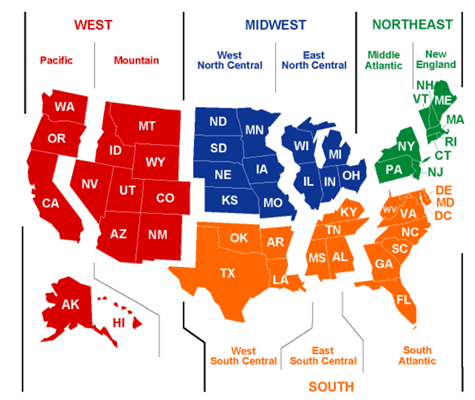
\includegraphics[scale=0.75]{images/natural_gas_census_regions.png}
    \caption{Census regions for natural gas fixed charges}
    \label{fig:natural_gas_census_regions}
\end{figure}

2023 EIA data was used for the price, consumption, and number of consumers.

Natural gas prices from the EIA 2023 "Residential Price" Data Series were used for the "Annual" period(\cite{EIA_natural_gas_prices}). Some 2024 prices were available, but 2023 prices were used to ensure consistency across the data. This data was released in May 2025.

The natural gas consumption values came from the EIA 2023 "Volumes Delivered to Residential" data series for the "Annual" period(\cite{EIA_natural_gas_consumption}). Like natural gas prices, some 2024 values were available, but 2023 consumption values were used and this data was also released in May 2025.

The number of consumers per state used in this ResStock dataset were released in April 2025(\cite{EIA_natural_gas_consumers}). The data series used was the "No. of Residential Consumers". None of the states had 2024 data available at the time of writing, therefore all states and Washington D.C. used 2023 data.

The volumetric rate for each state and Washington D.C. is seen in the following equation.
\begin{equation}
\label{eq:volumetric_natural_gas_rate}
\text{Volumetric natural gas rate} = \frac{(\text{Consumption} \times \text{price}) - (\text{Fixed cost per month} \times 12 \text{ months} \times \text{Number of consumers})}{(\text{Consumption} \times \text{Price})}
\end{equation}

The rates ranged from \$0.76\/therm in North Dakota to \$4.63\/therm in Hawaii.

The full year natural gas bill was then calculated for each modeled dwelling unit using its natural gas consumption and state volumetric rate.
\begin{equation}
\label{eq:natural_gas_bill_calc}
\text{Annual natural gas bill} = (\text{Fixed cost per month} \times 12 \text{ months}) + (\text{Natural gas consumption} \times \text{Volumetric natural gas rate})
\end{equation}

If the dwelling unit had no natural gas consumption in the baseline, but then received a gas furnace, then the dwelling unit had natural gas charges only in the upgrade scenario. In all other cases, a dwelling unit that originally had no natural gas consumption will not have any natural gas consumption in any other upgrade scenarios. If the dwelling unit had natural gas in the baseline, but then a measure upgrade caused there to be no gas, there is no natural gas bill for that measure upgrade. Fixed charges are applied monthly if there is a gas connection or gas consuming appliance, even if the month had zero natural gas consumption.

\subsection{Residential Propane Bills}
Propane costs for all states except for Alaska were taken from the 5/21/2025 release of the Weekly Heating Oil and Propane Prices from the EIA(\cite{EIA_propane_prices}).The data series was “Residential Propane” and the period was “Weekly”. Weekly prices from December 2024 through February 2025 were averaged together. State prices were used first if available. If state values were not available, Petroleum Administration for Defense District (PADD) values were used. If PADD values were not available, the U.S. weekly prices were used. PADD regions are reproduced below for clarity(\cite{EIA_padd_definitions}).

\begin{longtable}{ |p{3cm}|p{8cm}| }
\caption{PADD regions} \label{table:PADD_regions} \\
\toprule\noalign{}
\textbf{PADD Region} & \textbf{States} \\
\midrule\noalign{}
\endhead
\bottomrule\noalign{}
        PADD 1A (New England) & Connecticut, Maine, Massachusetts, New Hampshire, Rhode Island, Vermont \\ \hline
        PADD 1B (Central Atlantic) & Delaware, District of Columbia, Maryland, New Jersey, New York, Pennsylvania \\ \hline
        PADD 1C (Lower Atlantic) & Florida, Georgia, North Carolina, South Carolina, Virginia, West Virginia \\ \hline
        PADD 2 (Midwest) & Illinois, Indiana, Iowa, Kansas, Kentucky, Michigan, Minnesota, Missouri, Nebraska, North Dakota, Ohio, Oklahoma, South Dakota, Tennessee, Wisconsin \\ \hline
        PADD 3 (Gulf Coast) & Alabama, Arkansas, Louisiana, Mississippi, New Mexico, Texas \\ \hline
        PADD 4 (Rocky Mountain) & Colorado, Idaho, Montana, Utah, Wyoming \\ \hline
        PADD 5 (West Coast) & Alaska, Arizona, California, Hawaii, Nevada, Oregon, Washington \\ \hline
\end{longtable}

States using averaged U.S. weekly prices are Arizona, California, Oregon, Washington, Hawaii, and Nevada. States using their PADD region prices include Louisiana, New Mexico, West Virginia, South Carolina, Wyoming, and the District of Columbia. All other states, aside from Alaska, used their own state prices from EIA. Prices ranged from \$1.64/gallon in Iowa to \$4.75/gallon in Florida.

Propane prices for Alaska were taken from the Alaska Housing Finance Corporation's Fuel Survey dated 2025-03-01(\cite{AHFC_survey}).This data is typically used in the AkWarm energy modeling software. Taxes were included in the prices. The Alaska state average price using this survey is \$8.11/gallon.

Propane bills often have fixed or static charges. However, due to lack of national information on these values, these fixed or static charges were assumed to be zero.

\subsection{Residential No. 2 Fuel Oil Bills}
No. 2 fuel oil prices for all states, except Alaska, were taken from the 5/21/2025 release of the Weekly Heating Oil and Propane Prices from the EIA(\cite{EIA_fuel_oil_prices}). The data series was “Residential Heating Oil” and the period was “Weekly”. Weekly prices from December 2024 through February 2025 were averaged together. State prices were used first, and if those were not available, PADD regions were used next and then U.S. prices. PADD regions are the same for No. 2 fuel oil and propane.

States using averaged U.S. weekly prices include Arizona, Arkansas, California, Colorado, Hawaii, Idaho, Louisiana, Mississippi, Montana, Nevada, New Mexico, Oregon, Texas, Utah, Washington, and Wyoming. States using their PADD prices include District of Columbia, Illinois, Florida, Georgia, Kansas, Missouri, North Dakota, Oklahoma, South Carolina, South Dakota, Tennessee, and West Virginia. All other states, aside from Alaska, used their own state prices. Prices ranged from \$2.75/gallon in Nebraska to \$4.02/gallon in Delaware.

Alaska prices come from the Alaska Fuel Price Report: Winter 2025(\cite{AK_community_affairs}). The average unsubsidized No. 2 heating fuel price of 93 communities was \$6.48/gallon, and this will be used for the whole state of Alaska. Notable exclusions from the Alaska Fuel Price Report data include Anchorage and Mat-Su. Please read the Alaska Fuel Price report for other relevant assumptions.

Heating fuel bills often have fixed or static charges. However, due to lack of national information on these values, these fixed or static charges were assumed to be zero.

\section{Energy Burden}
Energy burden is calculated as the ratio of two values from ResStock data. The first is the energy bill, which is calculated for each individual housing unit model in an analysis as described in the above section. The second is the representative household income, which is converted from income bin and other household characteristics described in Section \ref{resstock_input_energy_burden}. The energy burden is the energy bill total divided by the representative household income, typically expressed as a percentage. As the utility bill does not account for financial assistance such as LIHEAP, energy burden may be overestimated for low-income households who may qualify for those assistance. Additionally, the representative income is in 2019 USD, reflecting the vintage of PUMS used to derived the data. The dollar value of the utility bill is typically more recent and thus may not align with that of the income denominator.

When this field is available in public datasets, it begins with ``out.energy\_burden.``

\section{Schedules}
ResStock optionally outputs schedules into the timeseries files. These schedules include energy use schedules as fractions (0-1) and unavailable period schedules from HVAC, power outage, and vacancy periods.

\begin{customLongTable}{ |p{6.cm}|p{1.8cm}|p{8.2cm}| }
{ResStock schedule output field names, units, and descriptions} {tab:schedule_outputs}
{\textbf{Field Name} & \textbf{Units} & \textbf{Field Description}}
out.schedules\_ceiling\_fan & frac & Ceiling fan energy use schedule. \\ \hline
out.schedules\_clothes\_dryer & frac & Clothes dryer energy use schedule. \\ \hline
out.schedules\_clothes\_washer & frac & Clothes washer energy use schedule. \\ \hline
out.schedules\_cooking\_range & frac & Cooking range and oven energy use schedule. \\ \hline
out.schedules\_dishwasher & frac & Dishwasher energy use schedule. \\ \hline
out.schedules\_hot\_water\_clothes\_washer & frac & Clothes washer hot water use schedule. \\ \hline
out.schedules\_hot\_water\_dishwasher & frac & Dishwasher hot water use schedule. \\ \hline
out.schedules\_hot\_water\_fixtures & frac & Fixtures (sinks, showers, baths) hot water use schedule. \\ \hline
out.schedules\_lighting\_garage & frac & Garage lighting energy use schedule. \\ \hline
out.schedules\_lighting\_interior & frac & Interior lighting energy use schedule. \\ \hline
out.schedules\_no\_space\_cooling & 0,1 & Cooling unavailable period. \\ \hline
out.schedules\_no\_space\_heating & 0,1 &  Heating unavailable period. \\ \hline
out.schedules\_occupants & frac & Occupant heat gain schedule. \\ \hline
out.schedules\_plug\_loads\_other & frac & Other plug load energy use schedule. \\ \hline
out.schedules\_plug\_loads\_tv & frac & Television plug load energy use schedule. \\  \hline
out.schedules\_power\_outage & 0,1 & Power outage unavailable period. \\ \hline
out.schedules\_vacancy & 0,1 & Vacancy unavailable period. \\
\end{customLongTable}

\section{Electrical Panels} \label{sec:output_panels}
For electrical panel, occupied capacity and breaker spaces are tabulated by end use. The total occupied capacity and spaces are calculated as well as their headroom, or the amount of capacity or space left unused.  In public ResStock datasets, these fields are prefixed with ``out.electric\_panel`` and described in \ref{tab:panels}.
For capacity, the total occupied load (W) can be calculated using different methods and will be labeled accordingly. In the public datasets, results are available for the 2023 load-based (NEC 220.83) method only for existing dwellings. See Section \ref{sec:input_panels} for the method description. The occupied capacity (A) is converted from occupied load (W) by dividing by 240V, the panel voltage, and then subtracted from the input field ``in.electrical\_panel\_service\_rating``'' (A) to get the headroom capacity (A).
The headroom capacity is used to determine capacity constraint – the panel is considered capacity-constrained if headroom is negative and unconstrained otherwise. This outcome is useful to account for any additional costs needed to resolve the constraint, such as through an electrical panel or service upgrade, or by using lower power appliances as an alternative.
Users are encouraged to calculate the capacity constraint on their own to reflect their desired margin of error.

For breaker space, total rated count is labeled as an input metric in table \ref{table:hc_output_fields}. This is actually derived from the breaker space headroom, which is probabilistically assigned based on the panel ampacity rating and other housing characteristics, and a tabulation of electrical equipment in the baseline home. In the upgrade simulations, the total breaker space count is carried over from the baseline simulation and the headroom count is recalculated according to the content of the upgrade package. See Section \ref{sec:input_panels} for details.
For ease of interpretation by mirroring the structure of the capacity metrics, total breaker space count is labeled as an input just like the panel service rating. All occupied and headroom tabulations are labeled as outputs.
Breaker space headroom is used to calculate the space constraint, which exists when the headroom count is negative. The overall panel constraint is summarized into "no constraint", "space constrained only", "capacity constrained only", or "capacity and space constrained".

All results should be interpreted with uncertainty in mind, even if they look reasonable. The prediction of the panel service rating and headroom space do not account for all electrical and connected loads in the model. As a result, the capacity headroom can be negative for a model in the baseline, although it is uncommon.
This can be interpreted as the house already being constrained prior to any upgrade and is consistent with anecdotal observations that some houses do trip their breakers often, an indication of a capacity shortfall.
On the otherhand, the breaker space headroom in the baseline can never be negative because our modeling approach prevents this by sampling a non-negative headroom count directly. This is also consistent with the physical constraint of breaker space.

\begin{customLongTable}{ |p{6cm}|p{1.5cm}|p{7.5cm}| }
        {ResStock electrical panel output field names, units, and descriptions} {tab:panels}
        {\textbf{Field Name} & \textbf{Units} & \textbf{Field Description}}
                out.params.panel\_load\_total\_load.2023\_nec\_existing\_dwelling\_load\_based..w & W & Total service feeder load calculated per selected NEC method \\ \hline
                out.params.panel\_load\_occupied\_capacity.2023\_nec\_existing\_dwelling\_load\_based..a & A & Total capacity occupied on the panel, calculated as total load (W) divided by panel voltage (240V) \\ \hline
                out.params.panel\_load\_headroom\_capacity.2023\_nec\_existing\_dwelling\_load\_based..a & A & Available capacity on the panel, calculated as panel service rating (A) minus total occupied capacity (A) \\ \hline
                out.params.panel\_load\_heating..w & W & Sum of space heating system and heat pump heating electric loads. For the load calculation, only the max of heating or cooling is used, not both \\ \hline
                out.params.panel\_load\_cooling..w & W & Sum of space cooling system and heat pump cooling electric loads. For the load calculation, only the max of heating or cooling is used, not both \\ \hline
                out.params.panel\_load\_hot\_water..w & W & Sum of water heating system electric loads, for electric only \\ \hline
                out.params.panel\_load\_clothes\_dryer..w & W & Sum of clothes dryer electric loads, for electric only \\ \hline
                out.params.panel\_load\_dishwasher..w & W & Sum of dishwasher electric loads \\ \hline
                out.params.panel\_load\_range\_oven..w & W & Sum of range/oven electric loads, for electric only \\ \hline
                out.params.panel\_load\_mech\_vent..w & W & Sum of mechanical ventilation electric loads \\ \hline
                out.params.panel\_load\_permanent\_spa\_heat..w & W & Sum of permanent spa heater electric load, for electric only \\ \hline
                out.params.panel\_load\_permanent\_spa\_pump..w & W & Sum of permanent spa pump electric loads \\ \hline
                out.params.panel\_load\_pool\_heater..w & W & Sum of pool heater electric loads \\ \hline
                out.params.panel\_load\_pool\_pump..w & W & Sum of pool pump electric loads \\ \hline
                out.params.panel\_load\_well\_pump..w & W & Sum of well pump electric loads \\ \hline
                out.params.panel\_load\_ev\_charging..w & W & Sum of electric vehicle charging equipment electric loads \\ \hline
                out.params.panel\_load\_other..w & W & Sum of other electric loads, including but not limited to lighting/general receptacles at 3 W/sqft, refrigerator, microwave, and garbage disposal \\ \hline
                out.params.panel\_breaker\_space\_occupied\_savings\_count & count & TODO \\ \hline
                out.params.panel\_breaker\_space\_occupied\_count & count & Total number of occupied spaces on the panel \\ \hline
                out.params.panel\_breaker\_space\_headroom\_count & count & Available spaces, calculated as total rated spaces minus occupied spaces \\ \hline
                out.params.panel\_breaker\_space\_heating\_count & count & Sum of heating system and heat pump heating occupied spaces \\ \hline
                out.params.panel\_breaker\_space\_cooling\_count & count & Sum of cooling system and heat pump cooling occupied spaces \\ \hline
                out.params.panel\_breaker\_space\_hot\_water\_count & count & Sum of water heating system occupied spaces \\ \hline
                out.params.panel\_breaker\_space\_clothes\_dryer\_count & count & Sum of clothes dryer occupied spaces \\ \hline
                out.params.panel\_breaker\_space\_dishwasher\_count & count & Sum of dishwasher occupied spaces \\ \hline
                out.params.panel\_breaker\_space\_range\_oven\_count & count & Sum of range/oven occupied spaces \\ \hline
                out.params.panel\_breaker\_space\_mech\_vent\_count & count & Sum of mechanical ventilation occupied spaces \\ \hline
                out.params.panel\_breaker\_space\_permanent\_spa\_heat\_count & count & Sum of permanent spa heater occupied spaces \\ \hline
                out.params.panel\_breaker\_space\_permanent\_spa\_pump\_count & count & Sum of permanent spa pump occupied spaces \\ \hline
                out.params.panel\_breaker\_space\_pool\_heater\_count & count & Sum of pool heater occupied spaces \\ \hline
                out.params.panel\_breaker\_space\_pool\_pump\_count & count & Sum of pool pump occupied spaces \\ \hline
                out.params.panel\_breaker\_space\_well\_pump\_count & count & Sum of well pump occupied spaces \\ \hline
                out.params.panel\_breaker\_space\_ev\_charging\_count & count & Sum of electric vehicle charging occupied spaces \\ \hline
                out.params.panel\_breaker\_space\_other\_count & count & Sum of other electric load occupied spaces \\ \hline

                out.params.panel\_constraint\_capacity.2023\_nec\_existing\_dwelling\_load\_based & bool & Whether electric panel is capacity-constrained per the given method, defined as when out.params.panel\_load\_headroom\_capacity.2023\_nec\_existing\_dwelling\_load\_based.a < 0 \\ \hline
                out.params.panel\_constraint\_breaker\_space & bool & Whether electric panel is space-constrained, defined as when out.panel.breaker\_space.headroom\_count < 0 \\ \hline
                out.params.panel\_constraint\_overall.2023\_nec\_existing\_dwelling\_load\_based & categorical & Summarize overall electric panel constraint per the given method as "no constraint", "space constrained only", "capacity constrained only", or "capacity and space constrained" \\ \hline

                out.params.panel\_load\_total\_load.2023\_nec\_existing\_dwelling\_load\_based..w.savings & W & For an upgrade measure only, total service feeder load reduced per selected NEC method \\ \hline
                out.params.panel\_load\_occupied\_capacity.2023\_nec\_existing\_dwelling\_load\_based.a.savings & A & For an upgrade measure only, total occupied capacity reduced per selected NEC method \\ \hline
                out.panel.breaker\_space.occupied\_count.savings & count & For an upgrade measure only, total number of occupied spaces reduced \\
\end{customLongTable}

\section{Other Outputs}

The ResStock workflow can optionally output any variable available in EnergyPlus. We regularly use this capability for a variety of purposes, including modeling improvement and validation, debugging, special purpose variables for specific projects, and additional variables to publish as part of public datasets.

Table \ref{tab:other_outputs} shows a list of output variables that are not covered in other headings in this section but that we have typically included in many of our recent public datasets, where they begin with ``out.x.''

\begin{customLongTable}{ |p{6cm}|p{1.5cm}|p{7.5cm}| }
{Other ResStock results output field names, units, and descriptions} {tab:other_outputs}
{\textbf{Field Name} & \textbf{Units} & \textbf{Field Description}}
        out.cooling\_unavailable\_period & & Cooling unavailable period. \\ \hline
        out.electricity.summer.peak.kw & kW & Maximum power value in Jun/Jul/Aug \\ \hline
        out.electricity.winter.peak.kw & kW & Maximum power value in Dec/Jan/Feb \\ \hline
        out.heating\_unavailable\_period & & Heating unavailable period. \\ \hline
        out.hot\_water.clothes\_washer.gal & gal & Hot water consumed by clothes washer \\ \hline
        out.hot\_water.dishwasher.gal & gal & Hot water consumed by dishwasher \\ \hline
        out.hot\_water.distribution\_waste.gal & gal & Hot water consumed by water distribution system (water remaining in the pipe) \\ \hline
        out.hot\_water.fixtures.gal & gal & Hot water consumed by showers, sinks, and baths \\ \hline
        out.params.size\_water\_heater..gal & gal & Size of water heater \\ \hline
        out.load.cooling.energy\_delivered..kbtu & kbtu & Total energy delivered by cooling system includes HVAC distribution losses \\ \hline
        out.load.cooling.peak..kbtu\_per\_hr & kbtu/hr & Maximum cooling load delivered by cooling system includes HVAC distribution losses \\ \hline
        out.load.heating.energy\_delivered..kbtu & kbtu & Total energy delivered by heating system includes HVAC distribution losses \\ \hline
        out.load.heating.peak..kbtu\_per\_hr & kbtu/hr & Maximum heating energy delivered by heating system includes HVAC distribution losses over a 60 min time period \\ \hline
        out.load.hot\_water.energy\_delivered..kbtu & kbtu & Total energy delivered by hot water system includes contributions by desuperheaters or solar thermal systems \\ \hline
        out.load.hot\_water.energy\_solar\_thermal..kbtu & kbtu & Total energy delivered by solar hot water system \\ \hline
        out.load.hot\_water.energy\_tank\_losses..kbtu & kbtu & Total energy lost by hot water system tanks \\ \hline
        out.unmet\_hours.cooling..hr & hr & Number of hours where the cooling setpoint is not maintained \\ \hline
        out.unmet\_hours.heating..hr & hr & Number of hours where the heating setpoint is not maintained \\ \hline
        out.unmet\_hours.ev\_driving..hr & hr & Number of EV driving that cannot be achieved due to lack of charge \\ \hline
        weight & n/a & the number of housing units the sample represents \\
\end{customLongTable}

For several of the outputs above, there is an associated savings or reduction column.
